%TC:ignore
\documentclass{article}
\usepackage{caption}
\usepackage{xcolor, colortbl}
\definecolor{RED}{HTML}{EB6231}
\definecolor{YELLOW}{HTML}{E29D26}
\definecolor{BLUE}{HTML}{5D80B4}
\definecolor{LIGHTGREY}{gray}{0.9}
\definecolor{BLUELINK}{HTML}{0645AD}
\definecolor{DARKBLUELINK}{HTML}{0B0080}
\definecolor{LIGHTGREEN}{HTML}{6ABD9B}
\definecolor{GREEN}{HTML}{8FB03E}
\definecolor{PURPLE}{HTML}{BE1E2D}
\definecolor{BROWN}{HTML}{A97C50}
\definecolor{PINK}{HTML}{DA1C5C}

\PassOptionsToPackage{hyphens}{url}
\usepackage{hyperref}
% for linking between references, figures, TOC, etc in the pdf document
\hypersetup{colorlinks,
    linkcolor=DARKBLUELINK,
    anchorcolor=DARKBLUELINK,
    citecolor=DARKBLUELINK,
    filecolor=DARKBLUELINK,
    menucolor=DARKBLUELINK,
    urlcolor=BLUELINK
} % Color citation links in purple
\PassOptionsToPackage{unicode}{hyperref}
\PassOptionsToPackage{naturalnames}{hyperref}

\usepackage[backend=biber,eprint=false,isbn=false,url=false,intitle=true,style=nature,date=year]{biblatex}
\addbibresource{references.bib}

\usepackage[margin=70pt]{geometry}
\usepackage{amssymb,amsfonts,amsmath,amsthm,mathtools}
\usepackage{lmodern}
\usepackage{bm,bbold,bbm}
\usepackage{verbatim}
\usepackage{float}
\usepackage{listings, enumerate, enumitem}
\usepackage{pgfplots, pgf,tikz}
\usepackage{blkarray}
\usepgfplotslibrary{fillbetween}
\pgfplotscreateplotcyclelist{colors}{LIGHTGREEN\\YELLOW\\RED\\GREEN\\BLUE\\}
\pdfinclusioncopyfonts=1

\renewcommand{\baselinestretch}{1.5}
\renewcommand{\arraystretch}{0.6}
\frenchspacing

\renewcommand{\thetable}{S\arabic{table}}
\renewcommand{\thefigure}{S\arabic{figure}}
\renewcommand{\theequation}{S.\arabic{equation}}

\newcommand{\der}{\text{d}}
\newcommand{\e}{\text{e}}
\newcommand{\Ne}{N_{\text{e}}}
\newcommand{\Multiply}{\cdot}
\newcommand{\CrossMultiply}{\bm{\times}}

% Genotype-Phenotype-Fitness
\newcommand{\NbrSites}{n}
\newcommand{\Geno}{\mathbb{G}}
\newcommand{\GenoDer}{\Geno^{\prime}}
\newcommand{\setNeighbors}{\mathcal{V}\left(\Geno\right)}
\newcommand{\Observed}{\mathcal{W}\left(\Geno\right)}
\newcommand{\PhenoDef}{x}
\newcommand{\PhenoParam}{\bm{\lambda}}
\newcommand{\PhenoParamSet}{\Lambda}
\newcommand{\GenoPhenoMap}{H_{\PhenoParam}}
\newcommand{\Pheno}{\GenoPhenoMap\left(\Geno\right)}
\newcommand{\PhenoDer}{\GenoPhenoMap\left(\GenoDer\right)}
\newcommand{\FitParam}{\bm{\theta}}
\newcommand{\FitParamSet}{\Theta}
\newcommand{\PhenoFitMapDef}{F}
\newcommand{\PhenoFitMap}{\PhenoFitMapDef_{\FitParam}}
\newcommand{\FitDef}{y}
\newcommand{\Fit}{\PhenoFitMap\left(\Pheno\right)}
\newcommand{\FitDer}{\PhenoFitMap\left(\PhenoDer\right)}
\newcommand{\Pfix}{P}
\newcommand{\SelCoeff}{S_{\PhenoParam, \FitParam}}
\newcommand{\mutmatrix}{r}
\newcommand{\Mutmatrix}{\bm{\mutmatrix}}
\newcommand{\exchan}{\rho}
\newcommand{\Exchan}{\bm{\exchan}}
\newcommand{\mutequi}{\pi}
\newcommand{\Mutequi}{\bm{\mutequi}}
\newcommand{\Pmut}{R_{\Exchan, \Mutequi}}
\newcommand{\PsubDef}{Q}
\newcommand{\PsubAll}{\PsubDef_{\Exchan, \Mutequi, \PhenoParam, \FitParam}}
\newcommand{\Psub}{\PsubDef_{\FitParam}}
\newcommand{\Normalize}{\mathcal{Z}_{\FitParam}\left(\Geno\right)}
\newcommand{\Diff}{D}

\begin{document}
    \part*{Supplementary materials}
    \tableofcontents
    \newpage

    \section{General formalism of the genotype to fitness map}\label{sec:general-formalism}

    DNA sequence evolution is modelled under an origin-fixation framework~\cite{mccandlish_modeling_2014}, meaning that the whole population is considered monomorphic and only the succession of fixation events are modeled.
    We consider the reconstructed ancestral DNA sequence as the reference sequence, and we model the evolution of the DNA sequence by substitutions of one nucleotide at a time occurring along the branch leading to the derived sequence.
    From the observed substitutions, we aim to retrieve information about the selection regime acting on the DNA sequence.
    Whether a mutation reaches fixation or not depends on the selection coefficient associated with the mutation (see section~\ref{sec:substitution-rate}), but determining the selection coefficient requires knowledge of the genotype to fitness map (see section~\ref{subsec:genotype-to-fitness-map}), which is decomposed into the genotype to phenotype map (see section~\ref{subsec:genotype-to-phenotype-map}) and the phenotype to fitness map (see section~\ref{subsec:phenotype-to-fitness-map}).

    \begin{center}
        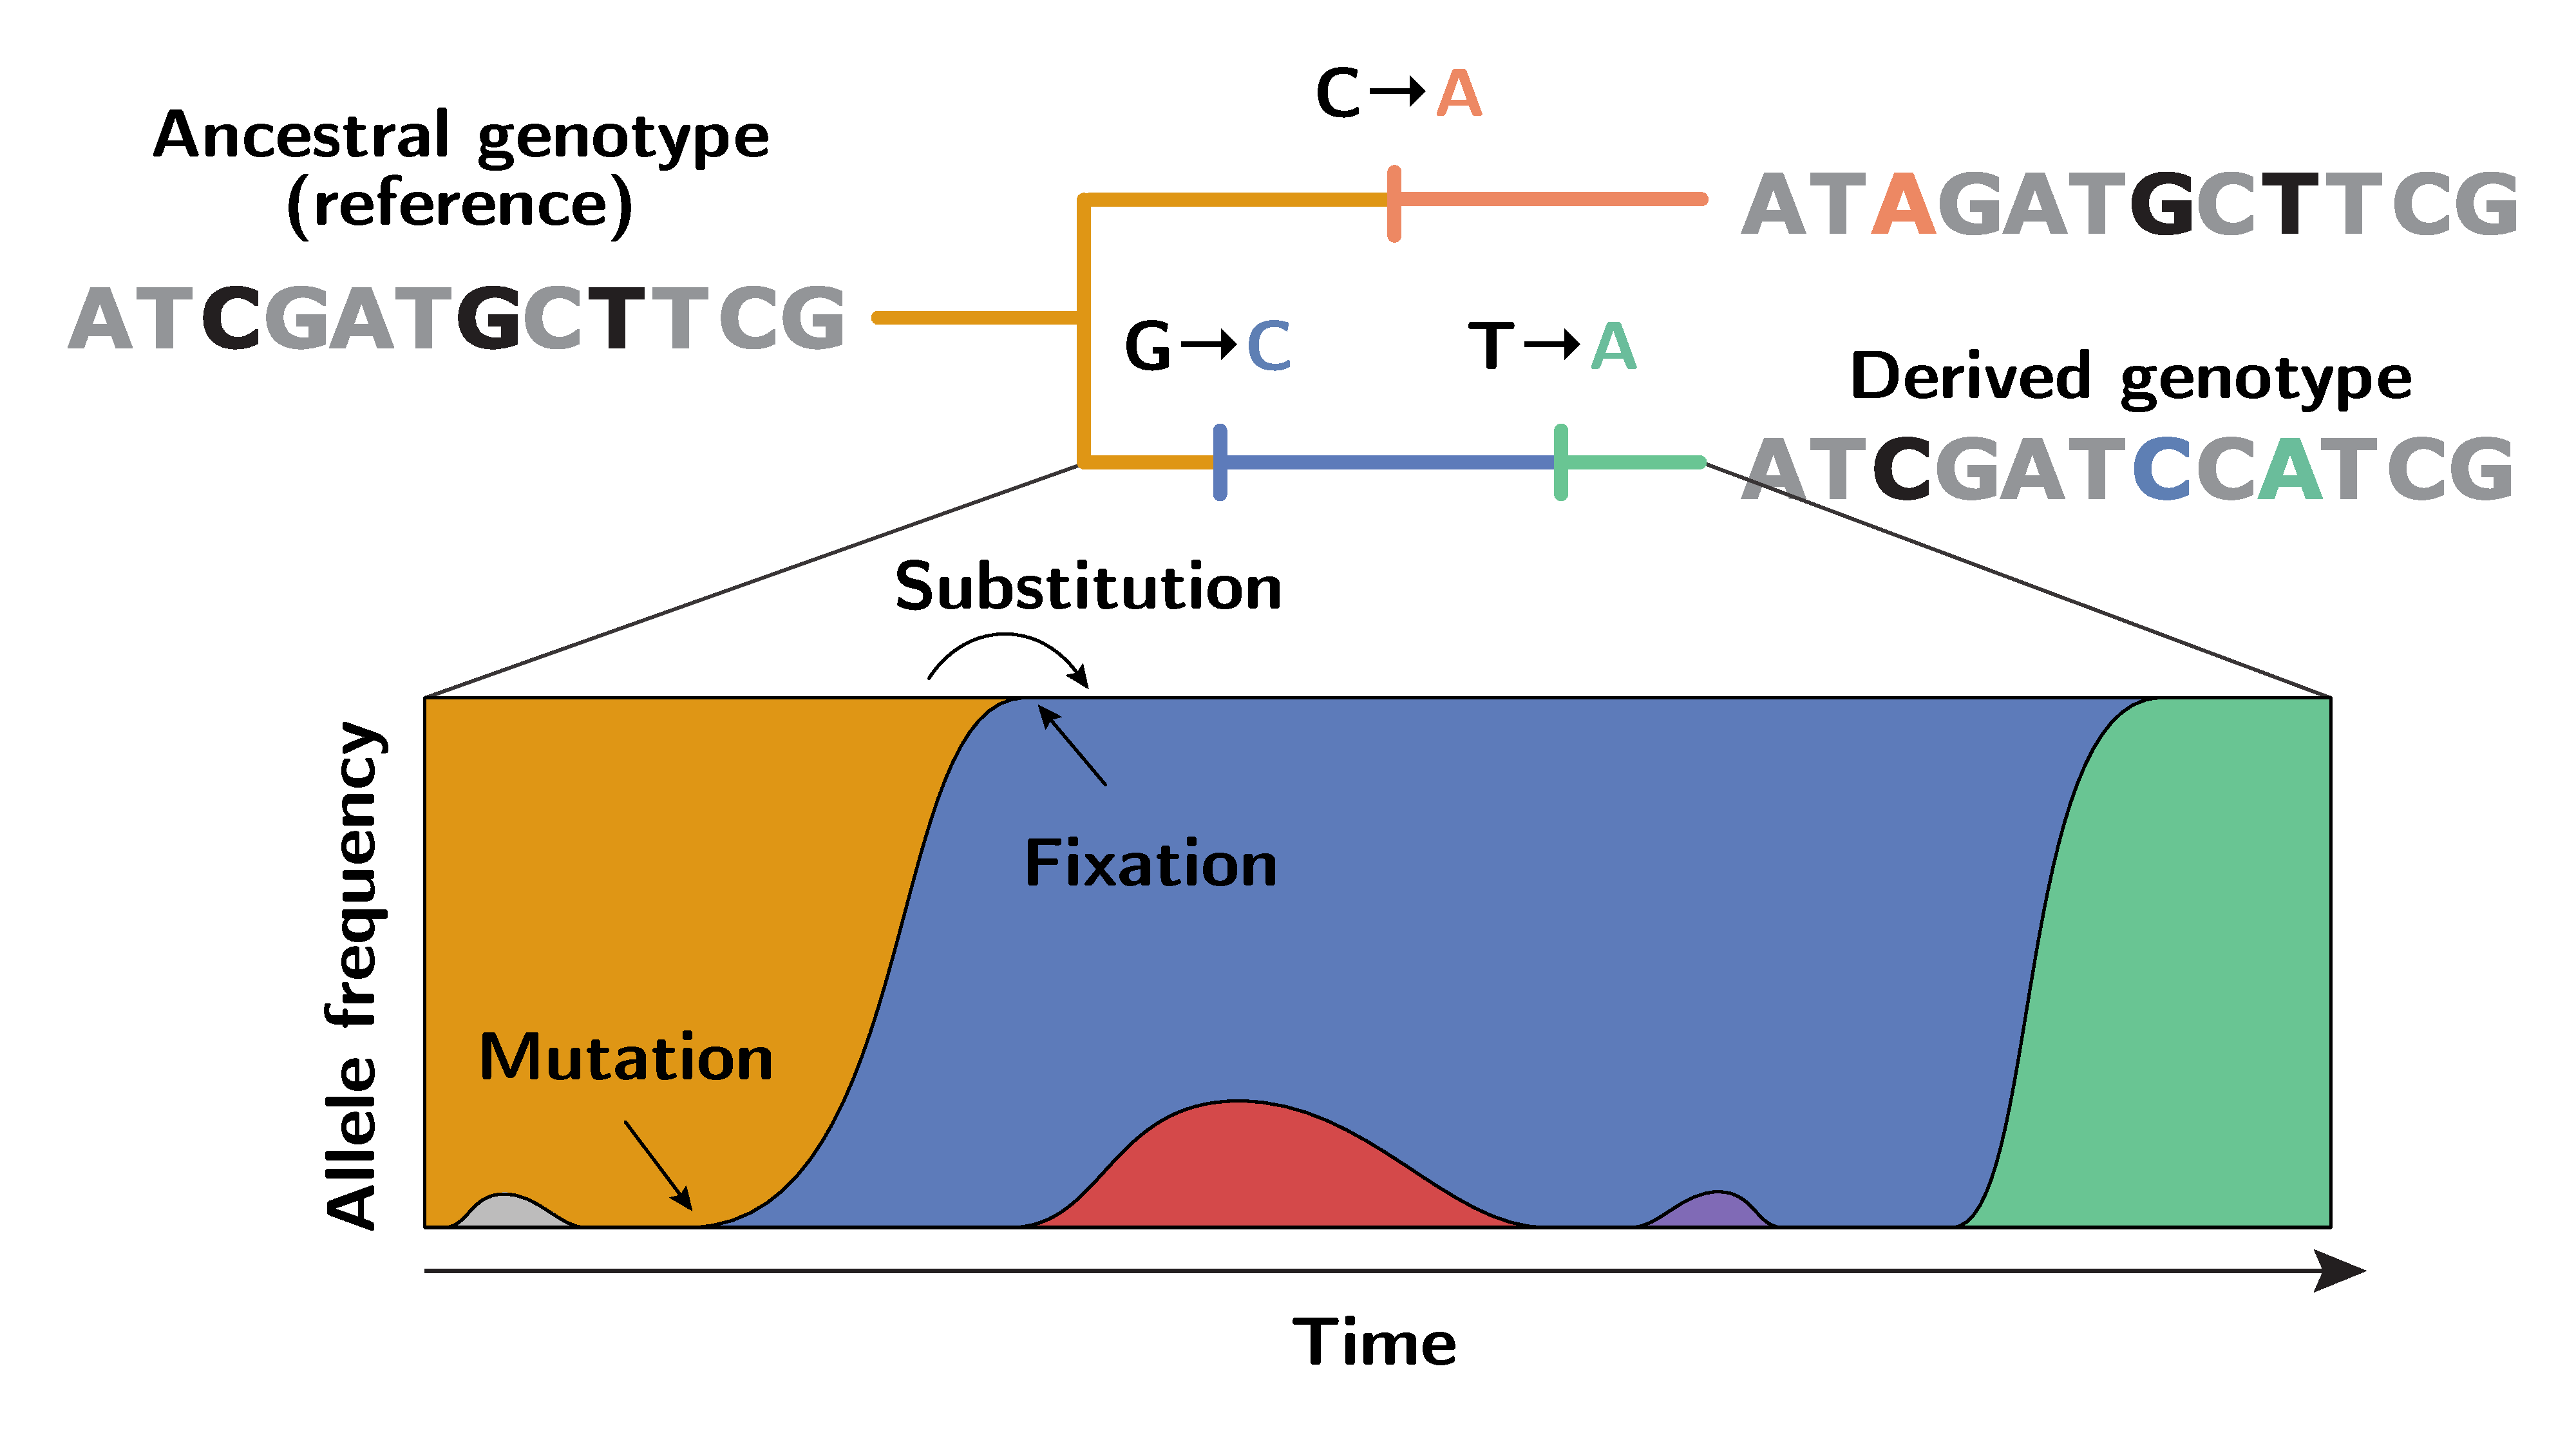
\includegraphics[width=0.6\linewidth, page=1]{substitutions.pdf}
        \label{fig:substitutions}
        \captionof{figure}{\textbf{Example of substitutions in the terminal lineage.} Substitutions are the product of mutation and fixation events, and since fixation events are determined by the selection coefficient, we can retrieve information about the selection regime from the observed substitutions.}
    \end{center}

    \subsection{Genotype to phenotype map}\label{subsec:genotype-to-phenotype-map}

    A genotype, $\Geno$, is a DNA sequence of $\NbrSites$ nucleotide sites:
    \begin{align}
        \Geno \in \left\{ A, C, G, T \right\}^{\NbrSites}.
    \end{align}

    In the example of figure~\ref{fig:substitutions}, the reference genotype is:
    \begin{align*}
        \Geno = \text{ATCGATGCTTCG}.
    \end{align*}

    The phenotype, $\PhenoDef$, is assumed to be a real number between $0$ and $1$, with the boundaries corresponding to the extreme phenotypes, while 0.5 corresponds to the reference phenotype:
    \begin{align}
        \PhenoDef \in \left[ 0, 1 \right].
    \end{align}

    And the genotype to phenotype map, $\Pheno$, is a function of the genotype ($\Geno$) and a set of parameters $\PhenoParam \in \PhenoParamSet$:
    \begin{align}
        \GenoPhenoMap : & \left\{ A, C, G, T \right\}^{\NbrSites} \to \left[ 0, 1 \right], \\
        & \Geno \mapsto \PhenoDef.
    \end{align}
    In the example of figure~\ref{fig:substitutions}, the phenotypes corresponding to ancestral sequences and the sequence after a substitution should be a real number between $0$ and $1$, such as for example:
    \begin{align*}
        \begin{dcases}
            \GenoPhenoMap (\text{ATCGAT\textbf{G}C\textbf{T}TCG} ) & = 0.5. \\
            \GenoPhenoMap (\text{ATCGAT{\color{BLUE}{\textbf{C}}}C\textbf{T}TCG} ) & = 0.813. \\
            \GenoPhenoMap (\text{ATCGAT\textbf{G}C{\color{LIGHTGREEN}{\textbf{A}}}TCG} ) & = 0.752.
        \end{dcases}
    \end{align*}

    In the following the genotype to phenotype map is assumed to be known, meaning that the phenotype is a deterministic function of the genotype and that the parameters $\PhenoParam$ are fixed.
    This representation is a general case, and we apply it to the binding affinity in two different ways in section~\ref{sec:application-to-binding-affinity}.

    \subsection{Phenotype to fitness map}\label{subsec:phenotype-to-fitness-map}
    The Wrightian fitness, $\FitDef$, is a positive real number giving the relative reproductive success.
    The phenotype to fitness map, $\Fit$, is a function of the phenotype ($\PhenoDef$) and a set of parameters $\FitParam \in \FitParamSet$:
    \begin{align}
        \PhenoFitMap : & \left[ 0, 1 \right] \to \mathbb{R}_{+}, \\
        & \PhenoDef \mapsto \FitDef.
    \end{align}
    In this case, the phenotype to fitness map is not assumed to be known.
    Here we use three fitness functions representing different selection regimes: no selection for the phenotype (section~\ref{subsubsec:no-selection}), stabilizing selection around the ancestral phenotype (section~\ref{subsubsec:stabilizing-selection}) and directional selection (section~\ref{subsubsec:directional-selection}).

    \subsubsection{No selection on the phenotype}
    \label{subsubsec:no-selection}
    In a case of no selection on the phenotype, all phenotypes have the same fitness and the fitness function is thus constant:
    \begin{align}
        \PhenoFitMapDef (\PhenoDef) = 1.
    \end{align}
    In such a case, the set of parameters is empty:
    \begin{gather}
        \FitParamSet = \emptyset.
    \end{gather}

    \subsubsection{Stabilizing selection around the ancestral phenotype}
    \label{subsubsec:stabilizing-selection}
    In the model of stabilizing selection around the ancestral phenotype, the fitness is maximal for the ancestral phenotype ($\PhenoDef = 0.5$), and decreases as the phenotype moves away from the optimum.
    We used a Beta distribution to model the fitness function:
    \begin{align}
        \PhenoFitMapDef_{\alpha} (\PhenoDef) = \frac {\Gamma (2 \alpha )}{\Gamma (\alpha )^2} \Multiply \PhenoDef^{\alpha -1} \Multiply (1-\PhenoDef)^{\alpha -1},
    \end{align}
    where $\Gamma$ is the gamma function:
    \begin{align}
        \Gamma (z)=\int _{0}^{\infty }t^{z-1} \Multiply e^{-t} \der t.
    \end{align}

    In this case, the fitness function is parameterized by a single parameter $\alpha$ and the parameter space is thus 1-dimensional:
    \begin{gather}
        \begin{cases}
            \FitParam = \alpha,\\
            \FitParamSet = [ 1 ; +\infty [
        \end{cases}
    \end{gather}
    Importantly, the case $\alpha = 1$ corresponds to the model of no selection on the phenotype (section~\ref{subsubsec:no-selection}), such that the two models are nested.

    \subsubsection{Directional selection}
    \label{subsubsec:directional-selection}
    In the directional selection model, the fitness is maximal at one of the extreme phenotypes and minimal at the other extreme.
    We used a Beta function to model the fitness function:
    \begin{align}
        \PhenoFitMapDef_{\alpha, \beta} (\PhenoDef) = \frac {\Gamma (\alpha +\beta )}{\Gamma (\alpha ) \Multiply \Gamma (\beta )} \Multiply \PhenoDef^{\alpha -1} \Multiply (1-\PhenoDef)^{\beta -1},
    \end{align}
    where $\Gamma$ is the gamma function:
    \begin{align}
        \Gamma (z)=\int _{0}^{\infty }t^{z-1} \Multiply e^{-t} \der t.
    \end{align}

    In this case, the fitness function is parameterized by two parameters $(\alpha, \beta)$ and the parameter space is 2-dimensional:
    \begin{gather}
        \begin{cases}
            \FitParam = (\alpha, \beta),\\
            \FitParamSet = \mathbb{R}_{+} \CrossMultiply \mathbb{R}_{+}.
        \end{cases}
    \end{gather}

    Importantly, the case where $1 \leq \alpha = \beta $ corresponds to the stabilizing selection model around the ancestral phenotype (section~\ref{subsubsec:stabilizing-selection}), such that the two models are nested.
    Because the model of no selection (section~\ref{subsubsec:no-selection}) is also nested in the stabilizing selection model, and the stabilizing selection model is nested in the directional selection model, the three models are nested.

    \begin{center}
        \begin{tikzpicture}
            \begin{axis}
                [
                width=0.6\textwidth,
                height=0.5\textwidth,
                cycle list name=colors,
                domain=0:1,
                samples=100,
                xlabel={Phenotype ($\PhenoDef$)},
                ylabel={Fitness ($\FitDef = \PhenoFitMap(\PhenoDef)$)},
                ymin=0.0, ymax=5.0,
                legend entries={Neutral,Stabilizing selection ($\PhenoFitMapDef_{2}$),Stabilizing selection ($\PhenoFitMapDef_{8}$), Directional selection ($\PhenoFitMapDef_{1, 5}$), Directional selection ($\PhenoFitMapDef_{5, 1}$)},
                legend cell align=left,
                minor tick num=2,
                axis x line=bottom,
                axis y line=left,
                legend style={at={(0.2,0.99)},anchor=north west}
                ]
                % Beta(1,1): Normalization constant is 1
                \addplot[dotted, line width=1.5pt, YELLOW] {1.0};
                % Beta(2,2): Normalization constant is 6
                \addplot[dashed, line width=2.0pt, GREEN] {6*x^(2-1)*(1-x)^(2-1)};
                % Beta(8,8): Normalization constant is 51480
                \addplot[dashed, line width=2.0pt, LIGHTGREEN] {51480*x^(8-1)*(1-x)^(8-1)};
                % Beta(1,5): Normalization constant is 5
                \addplot[line width=2.0pt, RED] {5*x^(1-1)*(1-x)^(5-1)};
                % Beta(5,1): Normalization constant is 5
                \addplot[line width=2.0pt, BLUE] {5*x^(5-1)*(1-x)^(1-1)};
            \end{axis}
        \end{tikzpicture}
        \captionof{figure}{\textbf{Phenotype to fitness map ($\bm{\PhenoFitMap}$).}
        The Wrightian fitness is a function parameterized by $\FitParam$.
        The fitness function is constant for the model of no selection on the phenotype, and follows a Beta distribution for the models of stabilizing selection around the ancestral phenotype and directional selection.}
        \label{fig:phenotype-to-fitness-map}
    \end{center}

    \subsection{Genotype to fitness map}\label{subsec:genotype-to-fitness-map}

    To summarize, the genotype ($\Geno$) is first mapped to a phenotype ($\PhenoDef$) using the genotype to phenotype map ($ \PhenoDef = \Pheno$).
    Then the phenotype is mapped to a fitness ($\FitDef$) using the phenotype to fitness map ($\FitDef = \PhenoFitMap (\PhenoDef)$).
    Altogether, the genotype to fitness map is given by the composition of the two maps:
    \begin{align}
        \Geno \xmapsto{\GenoPhenoMap} \PhenoDef \xmapsto{\PhenoFitMap} \FitDef.
    \end{align}
    The genotype to phenotype map ($\GenoPhenoMap$) is assumed to be known, the goal being to estimate the parameters of the phenotype to fitness map ($\PhenoFitMap$) that best explain the observed substitutions.
    Moreover, the goal is also to compare the model fit and select the best model of fitness function among the three models presented in the previous section: no selection for the phenotype (section~\ref{subsubsec:no-selection}), stabilizing selection around the ancestral phenotype (section~\ref{subsubsec:stabilizing-selection}) and directional selection (section~\ref{subsubsec:directional-selection}).

    \newpage

    \section{Substitution rate}\label{sec:substitution-rate}

    In the origin-fixation framework~\cite{mccandlish_modeling_2014}, the substitution rate from a sequence to another is given by the product of the mutation rate (section~\ref{subsec:mutation-rate}) and the fixation rate (section~\ref{subsec:fixation-rate}).

    Given the currently fixed sequence $\Geno$, we define $\setNeighbors$ as the set of all possible neighbors that are one nucleotide away from $\Geno$.
    For a sequence of $\NbrSites$ nucleotide sites, $\left| \setNeighbors \right| = 3 \NbrSites$, since each site has $3$ possible changes.
    By definition, $\setNeighbors$ is a subset of the set of all possible sequences of $\NbrSites$ nucleotide sites:
    \begin{align}
        \setNeighbors \subset \left\{ A, C, G, T \right\}^{\NbrSites}.
    \end{align}

    In the example of figure~\ref{fig:substitutions}, the set of neighbors of the sequence $\Geno$ is:
    \begin{align*}
        \Geno = \hspace{0.75em} & \text{ATCGATGCTTCG} \\
        \text{and } \setNeighbors = \{ & \text{{\color{PINK}{\textbf{C}}}TCGATGCTTCG}, \\
        & \text{{\color{PINK}{\textbf{G}}}TCGATGCTTCG}, \\
        & \text{{\color{PINK}{\textbf{T}}}TCGATGCTTCG}, \\
        & \text{A{\color{PINK}{\textbf{A}}}CGATGCTTCG}, \\
        & \text{A{\color{PINK}{\textbf{C}}}CGATGCTTCG}, \\
        & \quad \quad \quad \quad \quad \vdots  \\
        & \text{ATCGATGCTTC{\color{PINK}{\textbf{T}}}} \}
    \end{align*}

    \subsection{Mutation rate}\label{subsec:mutation-rate}
    The rate of mutation from the reference sequence $\Geno$ to a derived sequence $\GenoDer$ is given by the change of a single nucleotide.
    As such, it is defined only for the sequences that differ by a single nucleotide: $\GenoDer \in \setNeighbors$.
    We denote $\Diff(\Geno,\GenoDer)$ as the pair of nucleotides that differ between the reference sequence $\Geno$ and the derived sequence $\GenoDer$.

    As an example, the nucleotide change between the reference sequence $\Geno = \text{ATCG{\color{YELLOW}{\textbf{A}}}TGCTTCG}$ and the derived sequence $\GenoDer = \text{ATCG{\color{PINK}{\textbf{C}}}TGCTTCG}$ is the pair AC (from nucleotide A to nucleotide C):
    \begin{align*}
        \Diff \left( \text{ATCG{\color{YELLOW}{\textbf{A}}}TGCTTCG},\text{ATCG{\color{PINK}{\textbf{C}}}TGCTTCG} \right) = \text{{\color{YELLOW}{\textbf{A}}}{\color{PINK}{\textbf{C}}}}.
    \end{align*}

    Then, the mutation rate between a pair of nucleotides is given by the nucleotide rate matrix $\Mutmatrix$.
    In its most general form, $\Mutmatrix$ is a $4 \CrossMultiply 4$ rate matrix with rate of mutation from nucleotide $a \in \{A, C, G, T\}$ to nucleotide $b \in \{A, C, G, T\}$ denoted as $\mutmatrix_{ab} \in \mathbb{R}_{+}$, and the rate of mutation away from nucleotide $a$ denoted as $\mutmatrix_{aa} \in \mathbb{R}_{-}$:
    \begin{equation}
        \label{eq:mutrates}
        \Mutmatrix =
        \begin{blockarray}{ccccc}
            & A                           & C                       & G                       & T                       \\
            \begin{block}{c(cccc)}
                A & \quad \mutmatrix_{AA} \quad & {\mutmatrix_{AC}} \quad & {\mutmatrix_{AG}} \quad & {\mutmatrix_{AT}} \quad \\
                C & \quad {\mutmatrix_{CA}}     & \mutmatrix_{CC}         & {\mutmatrix_{CG}}       & {\mutmatrix_{CT}}  \quad  \\
                G & \quad {\mutmatrix_{GA}}     & {\mutmatrix_{GC}}       & \mutmatrix_{GG}         & {\mutmatrix_{GT}}   \quad  \\
                T & \quad {\mutmatrix_{TA}}     & {\mutmatrix_{TC}}       & {\mutmatrix_{TG}}       & \mutmatrix_{TT}    \quad    \\
            \end{block}
        \end{blockarray}
    \end{equation}
    By definition, the sum of the entries in each row of the nucleotide rate matrix $\Mutmatrix$ is equal to $0$, giving the diagonal entries for each nucleotide $a \in \{A, C, G, T\}$:
    \begin{equation}
        \mutmatrix_{aa} = - \sum\limits_{ b \neq a, b \in \{A, C, G, T\} } \mutmatrix_{ab}.\label{eq:diag-mutrates}
    \end{equation}
    For example, the mutation rate away from nucleotide A is given by the sum of the mutation rates from nucleotide A to the other nucleotides:
    \begin{align*}
        \mutmatrix_{AA} = - \left( \mutmatrix_{AC} + \mutmatrix_{AG} + \mutmatrix_{AT} \right).
    \end{align*}
    A particular case of nucleotide rate matrix is the generalized time-reversible (GTR), where $\Mutmatrix$ is parameterized by the nucleotide frequencies denoted $\Mutequi = (\mutequi_A , \mutequi_C , \mutequi_G , \mutequi_T)$, and the symmetric exchangeability rates between nucleotides denoted $\Exchan = \left( \exchan_{AC}, \exchan_{AG}, \exchan_{AT}, \exchan_{CG}, \exchan_{CT}, \exchan_{GT}\right)$~\cite{tavare_probabilistic_1986}.
    $\Mutequi$ is the equilibrium base frequency vector, giving the frequency at which each base occurs at each site and satisfying the following condition:
    \begin{align}
        \sum\limits_{a \in \{A, C, G, T\}} \mutequi_a = 1.
    \end{align}
    From the parameter $\Mutequi$ and $\Exchan$, the nucleotide GTR rate matrix is defined as:
    \begin{equation}
        \label{eq:gtr-mutrates}
        \Mutmatrix =
        \begin{blockarray}{ccccc}
            & A                                        & C                                        & G                                        & T                                        \\
            \begin{block}{c(cccc)}
                A & \quad \mutmatrix_{AA} \quad              & {\exchan_{AC}\Multiply \mutequi_C} \quad & {\exchan_{AG}\Multiply \mutequi_G} \quad & {\exchan_{AT}\Multiply \mutequi_T} \quad \\
                C & \quad {\exchan_{AC}\Multiply \mutequi_A} & \mutmatrix_{CC}                          & {\exchan_{CG}\Multiply \mutequi_G}       & {\exchan_{CT}\Multiply \mutequi_T} \quad \\
                G & \quad {\exchan_{AG}\Multiply \mutequi_A} & {\exchan_{CG}\Multiply \mutequi_C}       & \mutmatrix_{GG}                & {\exchan_{GT}\Multiply \mutequi_T} \quad \\
                T & \quad {\exchan_{AT}\Multiply \mutequi_A} & {\exchan_{CT}\Multiply \mutequi_C}       & {\exchan_{GT}\Multiply \mutequi_G}       & \mutmatrix_{TT}          \quad  \\
            \end{block}
        \end{blockarray}
    \end{equation}
    The diagonal entries are given by equation~\ref{eq:diag-mutrates}.
    Moreover, the vector of exchangeabilities $\Exchan$ is normalized such that the nucleotide GTR rate matrix satisfies the following condition:
    \begin{align}
        \sum\limits_{a \in \{A, C, G, T\}} - \mutequi_a \Multiply \mutmatrix_{aa} = 1.
    \end{align}
    This normalization ensures that the total rate of mutation at equilibrium from any nucleotide to any other nucleotide is equal to $1$.
    In our method, we assume the nucleotide rate matrix $\Mutmatrix$ to be a known GTR rate matrix (equation~\ref{eq:gtr-mutrates}) with the equilibrium base frequencies $\Mutequi$ and the exchangeabilities $\Exchan$ as parameters estimated independently on another dataset.
    We estimated such parameters at the chromosome level, such that the nucleotide rate matrix $\Mutmatrix$ is the same for all sites of the same chromosome.

    Altogether, the mutation rate from the reference sequence $\Geno$ to the derived sequence $\GenoDer$ is given by the function $\Pmut$, parameterized be the vector of exchangeabilities $\Exchan$ and the vector of equilibrium base frequencies $\Mutequi$ of the GTR rate matrix (equation~\ref{eq:gtr-mutrates}):
    \begin{align}
        \Pmut : &  \left\{ A, C, G, T \right\}^{\NbrSites} \CrossMultiply \left\{ A, C, G, T \right\}^{\NbrSites} \to \mathbb{R}_{+}, \\
        & \left( \Geno,\GenoDer\right) \mapsto \mutmatrix_{\Diff(\Geno,\GenoDer)} \text{ if }\GenoDer \in \setNeighbors\text{, }0\text{ otherwise}.
    \end{align}

    As an example, the mutation rate from the reference sequence $\Geno = \text{ATCG{\color{YELLOW}{\textbf{A}}}TGCTTCG}$ to the derived sequence $\GenoDer = \text{ATCG{\color{PINK}{\textbf{C}}}TGCTTCG}$ is given by the mutation rate from nucleotide A to nucleotide C:
    \begin{align*}
        \Pmut \left( \text{ATCG{\color{YELLOW}{\textbf{A}}}TGCTTCG},\text{ATCG{\color{PINK}{\textbf{C}}}TGCTTCG} \right) = \mutmatrix_{AC} = \exchan_{AC} \Multiply \mutequi_C.
    \end{align*}

    \subsection{Fixation rate}\label{subsec:fixation-rate}
    For each mutant sequence $\GenoDer \in \setNeighbors$, we can compute its Wrightian fitness as $\FitDer$.
    The selection coefficient $\SelCoeff \left( \Geno,\GenoDer\right)$ associated to a change is the difference between the Malthusian fitness (log of Wrightian fitness) of the derived sequence and the Malthusian fitness of the reference sequence.
    In other words, the selection coefficient is the log-ratio of the Wrightian fitness of the derived sequence ($\FitDer$) to the Wrightian fitness of the reference sequence ($\Fit$):
    \begin{align}
        \SelCoeff : & \left\{ A, C, G, T \right\}^{\NbrSites} \CrossMultiply \left\{ A, C, G, T \right\}^{\NbrSites} \to \mathbb{R}, \\
        & \left( \Geno,\GenoDer\right) \mapsto \log \left[ \frac{\FitDer}{\Fit} \right].
    \end{align}
    Because the phenotype of the reference sequence is $\GenoPhenoMap (\Geno) = 0.5$, the fitness of the reference sequence is $\Fit = \PhenoFitMap\left(0.5\right)$ and the selection coefficient from the sequence $\Geno$ to $\GenoDer$ simplifies to:
    \begin{align}
        \SelCoeff \left( \Geno,\GenoDer\right) & = \log  \left[ \frac{\FitDer}{\PhenoFitMap\left(0.5\right)} \right] \\
        & = \log \left[ \FitDer \right] - \log \left[ \PhenoFitMap\left(0.5\right) \right].
    \end{align}

    Then, as described in the origin-fixation framework~\cite{mccandlish_modeling_2014}, the rate of fixation for a mutation, $\Pfix$, is a function of the selection coefficient as:
    \begin{align}
        \Pfix : &  \mathbb{R} \to \mathbb{R}_{+}, \\
        & s \mapsto \dfrac{s}{1 - \e^{-s}}.
    \end{align}

    \begin{center}
        \captionof{figure}{Fixation rate ($\Pfix$)}
        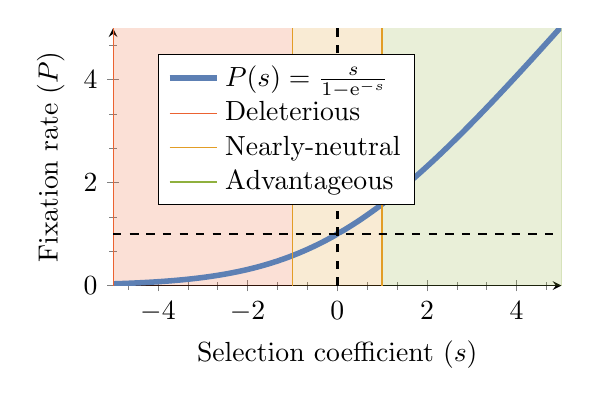
\begin{tikzpicture}
            \begin{axis}
                [
                width=0.6\textwidth,
                height=0.4\textwidth,
                ylabel={Fixation rate ($\Pfix$)},
                xlabel={Selection coefficient ($s$)},
                domain=-5:5,
                ymin=0.0, ymax=5.0,
                samples=200,
                legend entries={$\Pfix (s) = \frac{s}{1 - \e^{-s}}$,Deleterious,Nearly-neutral,Advantageous},
                legend cell align=left,
                minor tick num=2,
                axis x line=bottom,
                axis y line=left,
                legend style={at={(0.1,0.9)},anchor=north west}
                ]
                \addplot[line width=2.0pt, BLUE]{ x / (1 - exp(- x))};
                \addplot[name path=A, RED, line width=0.5pt] coordinates {(-5, 0) (-5, 5)};
                \addplot[name path=B, YELLOW, line width=0.5pt] coordinates {(-1, 0) (-1, 5)};
                \addplot[name path=D, GREEN, line width=0.5pt] coordinates {(5, 0) (5, 5)};
                \addplot[name path=C, YELLOW, line width=0.5pt] coordinates {(1, 0) (1, 5)};
                \addplot[black, dashed, line width=1.0pt]{1.0};
                \addplot[black, dashed, line width=1.0pt] coordinates {(0, 0) (0, 5)};
                \addplot[fill=RED, opacity=0.2] fill between[ of = A and B];
                \addplot[fill=YELLOW, opacity=0.2] fill between[ of = B and C];
                \addplot[fill=GREEN, opacity=0.2] fill between[ of = C and D];
            \end{axis}
        \end{tikzpicture}
        \label{fig:scaled-probability-of-fixation}
    \end{center}

    Altogether, the fixation rate from the reference sequence $\Geno$ to a derived sequence $\GenoDer \in \setNeighbors$ is obtained by first computing the selection coefficient $\SelCoeff \left( \Geno,\GenoDer\right)$, and then applying the fixation rate function $\Pfix$ to the selection coefficient:
    \begin{align}
        \Pfix \left( \SelCoeff \left( \Geno,\GenoDer\right)\right).
    \end{align}

    \newpage

    \subsection{Substitution rate as product of mutation and fixation rates}\label{subsec:substitution-rate}

    In the origin-fixation framework~\cite{mccandlish_modeling_2014}, the substitution rate from the reference sequence $\Geno$ to a derived sequence $\GenoDer \in \setNeighbors$, called $\Psub  \left( \Geno,\GenoDer\right)$, is given by the product of the mutation rate and the fixation rate:
    \begin{align}
        \PsubAll  \left( \Geno,\GenoDer\right) = \Pmut \left( \Geno,\GenoDer\right) \Multiply \Pfix \left( \SelCoeff \left( \Geno,\GenoDer\right)\right).
    \end{align}

    In details, the substitution rate from the reference sequence $\Geno$ to a derived sequence $\GenoDer \in \setNeighbors$ depends on the several parameters: the nucleotide GTR rate matrix ($\Exchan$ and $\Mutequi$, section~\ref{subsec:mutation-rate}), the genotype to phenotype map ($\PhenoParam$, section~\ref{subsec:genotype-to-phenotype-map}), and the phenotype to fitness map ($\FitParam$, section~\ref{subsec:phenotype-to-fitness-map}).

    \section{Likelihood of the data}\label{sec:likelihood-of-the-data}
    Now, we consider a set of observed substitutions $\Observed \subset \setNeighbors$ away from the ancestral sequence $\Geno$.
    Importantly, even if several substitutions are observed along the terminal branch, we cannot know the order of the substitutions and the time at which they occurred.
    As such, the substitutions are considered as independent events and thus a sample from the set of neighbor sequences $\setNeighbors$.

    In the example of figure~\ref{fig:substitutions}, the set of observed substitutions $\Observed$ away from the sequence $\Geno$ is:
    \begin{align*}
        \Geno = \hspace{0.75em} & \text{ATCGATGCTTCG} \\
        \text{and } \Observed = \{ & \text{ATCGAT{\color{PINK}{\textbf{C}}}CTTCG}, \\
        & \text{ATCGATGC{\color{PINK}{\textbf{A}}}TCG} \}
    \end{align*}

    In the following, because we assume the parameters of the nucleotide GTR rate matrix ($\Exchan$, $\Mutequi$, section~\ref{subsec:mutation-rate}) and of the genotype to phenotype map ($\PhenoParam$, section~\ref{subsec:genotype-to-phenotype-map}) to be known and fixed, they will be kept silent in the notation.
    Any function will be denoted solely as a function of the phenotype to fitness map: $\FitParam$ (section~\ref{subsec:phenotype-to-fitness-map}).
    For example, the substitution rate from the reference sequence $\Geno$ to a derived sequence $\GenoDer \in \setNeighbors$ will be denoted as $\Psub \left( \Geno,\GenoDer \right)$ instead of $\PsubAll \left( \Geno,\GenoDer \right)$.

    \subsection{Expected number of substitutions}\label{subsec:expected-number-of-substitutions}
    If the mutation rate per generation is constant and equals to $\mu$, and that the number of generations that occurred along the branch leading to the derived sequence is $t$, the expected number of substitutions that occurred along the branch, $q$ is given by:
    \begin{align}
        q = \mu \Multiply t \Multiply \sum_{\GenoDer \in \setNeighbors} \Psub \left( \Geno,\GenoDer \right).
    \end{align}

    However, because we don't know nor $\mu$ neither $t$, we cannot know the expected number of substitutions that would occur along the branch.
    In other word, the signal we are retrieving is not about the number of substitutions that occurred along the branch.
    Instead, the signal we are retrieving is about the phenotypic effect of the substitutions, whether they reflect the phenotypic effect of all possible mutations or only a subset of them.

    \subsection{Probability of an observed substitution}\label{subsec:probability-of-an-observed-substitution}
    First, we denote $\Normalize$ as the sum of substitution rates ($ \Psub $) for all possible neighbors ($\GenoDer \in \setNeighbors$) of the reference sequence $\Geno$:
    \begin{align}
        \Normalize = \sum_{\GenoDer \in \setNeighbors} \Psub \left( \Geno,\GenoDer \right).
    \end{align}
    This normalization factor $\Normalize$ depends explicitly on the reference sequence $\Geno$ and the parameters of the phenotype to fitness map ($\FitParam$).
    Then, for any observed substitution $\GenoDer \in \Observed$, we can compute the probability that such substitution has occurred among all possible substitutions as its substitution rate divided by the normalization factor:
    \begin{align}
        \dfrac{\Psub \left( \Geno,\GenoDer \right)}{\Normalize}.
    \end{align}

    This probability is high when the observed substitution is matching the most likely substitutions to have occurred among all neighbors of the reference sequence.
    This occurs when the model of fitness function $\PhenoFitMap$ give high probabilities to the one observed substitution, but low probabilities to the unobserved substitutions.

    \subsection{Likelihood of the observed substitutions}\label{subsec:likelihood-of-the-data}
    The data consists of the reference sequence $\Geno$ and the set of observed substitutions $\Observed \subset \setNeighbors$ away from the reference sequence.
    Each observed substitution $\GenoDer \in \Observed$ is considered an independent event and a sample from the set of all possible substitutions $\setNeighbors$.
    The likelihood of the data, denoted $\mathcal{L} (\Observed, \Geno | \FitParam )$, is computed as the product of the probabilities for each observed substitution:
    \begin{align}
        \mathcal{L} (\Observed, \Geno | \FitParam ) & = \prod_{\GenoDer \in \Observed} \dfrac{\Psub \left( \SelCoeff \left( \Geno,\GenoDer\right)\right)}{\Normalize}.
    \end{align}

    The likelihood of the data is thus total probability of the observed substitutions to be sampled from the set of all possible substitutions.
    As such, the likelihood is high when in general the observed substitutions are matching the most likely substitutions to have occurred among all neighbors of the reference sequence.
    This occurs when the model of fitness function $\PhenoFitMap$ give high probabilities to the observed substitutions, but low probabilities to the unobserved substitutions.

    In practice, $\mathcal{L} (\Observed, \Geno | \FitParam )$ is computed in log-space to avoid numerical errors:
    \begin{align}
        \log \left[ \mathcal{L} (\Observed, \Geno | \FitParam ) \right] & = \log \left[  \prod_{\GenoDer \in \Observed} \dfrac{\Psub \left( \Geno,\GenoDer\right)}{\Normalize} \right] \\
        & = \sum_{\GenoDer \in \Observed} \log \left[ \dfrac{ \Psub \left( \Geno,\GenoDer \right)}{\Normalize} \right] \\
        & = \sum_{\GenoDer \in \Observed} \left(  \log \left[ \Psub \left( \Geno,\GenoDer \right)\right] - \log \left[ \Normalize \right] \right) \\
        & = \sum_{\GenoDer \in \Observed} \left(  \log \left[ \Psub \left( \Geno,\GenoDer \right)\right] \right) - | \Observed | \Multiply \log \left[ \Normalize \right].
    \end{align}

    The parameter $\FitParam$ are estimated by maximizing $\mathcal{L} (\Observed, \Geno | \FitParam )$ with the Nelder-Mead algorithm.

    \subsection{Approximation by binning}\label{subsec:approximation-by-binning}
    The number of possible neighbors ($\left| \setNeighbors \right| = 3 \NbrSites$) is quite large, and the computation of the likelihood of the data requires computing the substitution rate for each of them.
    To reduce the computational cost, we can approximate the normalization factor by binning the neighbors with similar phenotypic effects.
    The number of bins is a fixed number, and each mutation and substitution is assigned to a bin based on the phenotypic effect of the change.
    The selection coefficient is thus computed only once per bin, reducing significantly the number of computations.

    \section{Application to binding affinity}\label{sec:application-to-binding-affinity}

    For a given DNA sequence, the binding affinity of a transcription factor is obtained via machine learning models.
    The binding affinity is a continuous variable, with high values corresponding to strong binding and low values corresponding to weak binding.
    But, the binding affinity is not constrained to be in the interval $[0, 1]$, hence we need to regularize the binding affinity to be in the unit interval.
    Moreover, the phenotype of the ancestral sequence must be 0.5.

    \subsection{Regularization of the phenotype map}\label{subsec:regularization-of-the-phenotype-map}
    The simplest way to regularize the binding affinity is to normalize by the extremal values, keeping the reference sequence at the center.

    \subsection{Quantization of the phenotype map}\label{subsec:quantization-of-the-phenotype-map}
    Another way to regularize the binding affinity is to quantize the binding affinity into a discrete number of bins.
    The binding affinity is then mapped to a discrete value corresponding to the bin in which it falls.

    \printbibliography
\end{document}